%%-*-latex-*-

\vspace*{\stretch{1}}

\begin{figure}[H] \centering
\fbox{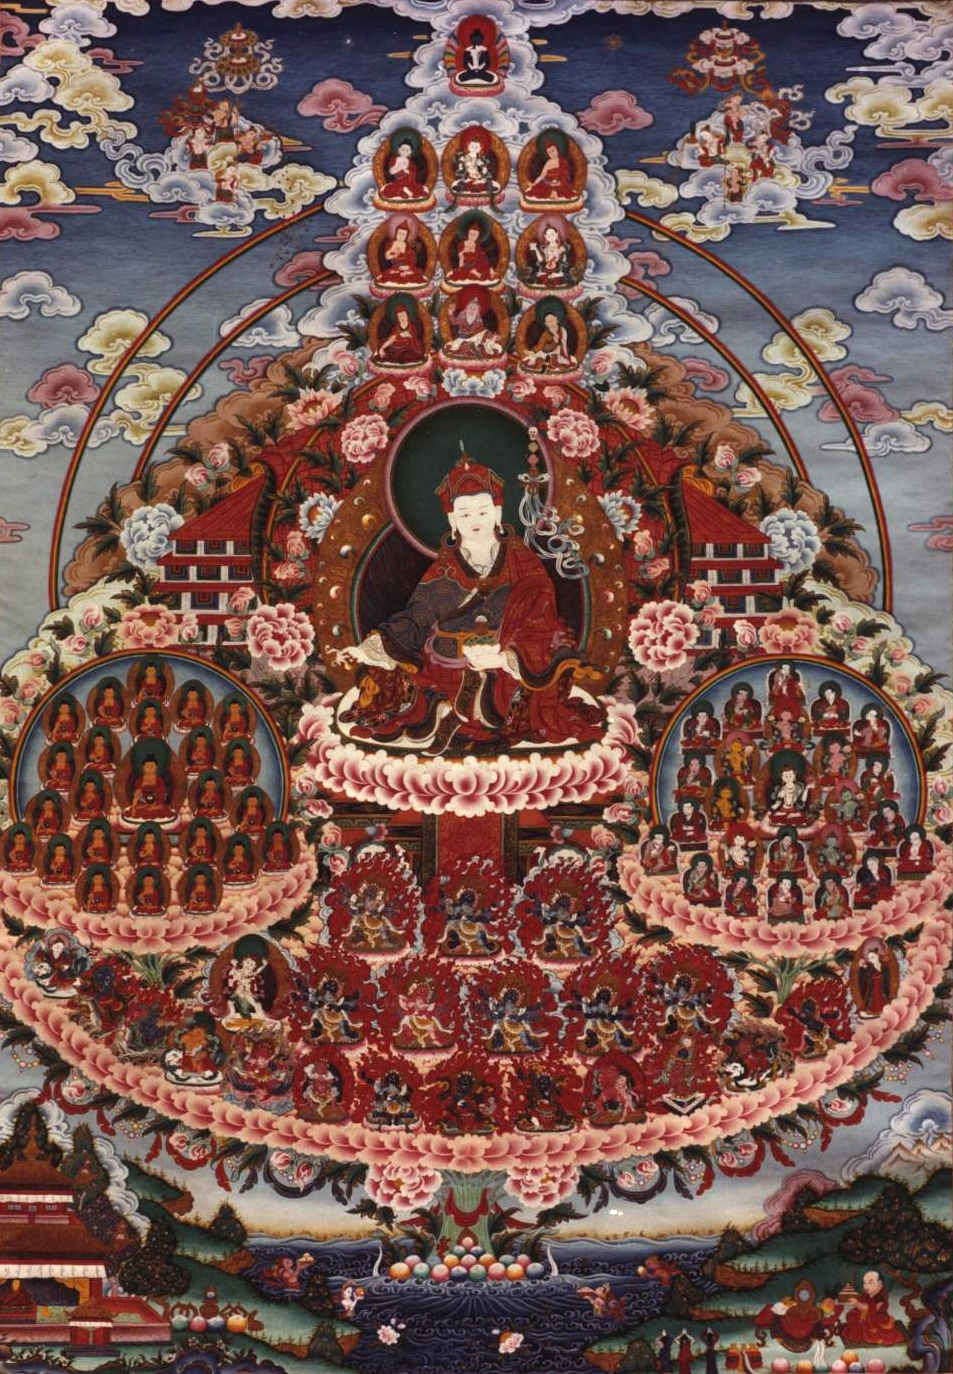
\includegraphics[scale=0.7]{refuge_tree.eps}}
\scaption{L'arbre de la lign�e Tersar}
\end{figure}

\vspace*{\stretch{1}}

\pagebreak

\titlesec{Refuge, aspiration d'�veil et offrande}
\addcontentsline{toc}{section}{\protect\numberline{}Refuge, aspiration
  d'�veil et offrande}

\bigskip\bigskip

\begin{tabbing}
\=\stib{'di bzung byang chub snying po ma thob bar\notsheg:}\\
\>\lit{di}--------------\=\lit{sung} \=\lit{jangchub} \=\lit{nyingpo}
\=\lit{ma}-\=\lit{thob} \ \=\lit{bra}\\
\>\lex{maintenant} \>\lex{depuis} \>\lex{�veil} \>\lex{c{\oe}ur}
\>\lex{pas} \>\lex{atteint} \>\lex{tant que}\\
\>\trans{D�sormais et jusqu'� ce que j'atteigne le c{\oe}ur de l'�veil,}\\
\>\stib{bla ma dkon mchog gsum la skyabs su mchi\notsheg:}\\
\=\lit{lama} \=\lit{k�nchog} \=\lit{sum} \=\lit{la} \=\lit{kyab su chi}\\
\>\lex{ma�tre} \>\lex{pr�cieux} \>\lex{trois} \>\lex{en}
\>\lex{je prends refuge}\\
\>\trans{je prends refuge dans le ma�tre et les Trois
Joyaux.}\sendnote{Les Trois Joyaux (\emph{triratna}) sont le
  Bouddha, la voie qu'il a montr�e (\emph{dharma}) et la
  communaut� (monastique et la�que r�unies, skt. \emph{sa\.{n}gha})
  qui la parcourt.}\\
\>\stib{da nas bzung ste 'khor ba ma stong bar\notsheg:}\\
\=\lit{da-ne}-----\=\lit{sung-te} \=\lit{khorwa} \quad \
\=\lit{ma}-\=\lit{tong} \=\lit{bra}\\
\>\lex{maintenant} \>\lex{depuis} \>\lex{\emph{sa\d{m}s\a={a}ra}}
\>\lex{non} \>\lex{vide} \>\lex{tant que}\\
\>\trans{D�sormais et tant que les mondes seront peupl�s,}\\
\>\stib{ma gyur sems can kun gyi phan bde bsgrub\notsheg:}\\
\>\lit{ma}---\=\lit{gyur} \quad \ \=\lit{semchen} \=\lit{k�n}-\=\lit{gyi}
\=\lit{phen}---\=\lit{de} \qquad \=\lit{drub}\\
\>\lex{m�re} \>\lex{(ayant) �t�} \>\lex{�tres} \>\lex{tous} \>\lex{de}
\>\lex{b�n�fice} \>\lex{bonheur} \>\lex{accomplir}\\
\>\trans{j'{\oe}uvrerai au bonheur des �tres, mes anciennes m�res.}
\end{tabbing}

\rep{� r�citer trois fois les mains jointes en pri�re (ou une fois en
  se prosternant).}

\begin{tabbing}
\=\stib{tshe rabs kun gyi lus dang longs spyod dpal\notsheg:}\\
\>\lit{tshe}-\=\lit{rab} \quad \ \ \=\lit{k�n}-\=\lit{gyi} \=\lit{l�}
\ \ \=\lit{dang} \=\lit{long} \=\lit{ch�} \=\lit{pel}\\
\>\lex{vies} \>\lex{succession} \>\lex{tous} \>\lex{de} \>\lex{corps}
\>\lex{et} \>\lex{joies} \>\lex{biens} \>\lex{honneurs}\\
\>\trans{Dans ma vie et les suivantes, corps, biens et honneurs,}\\
\>\stib{tshogs gnyis rdzogs phyir dkon mchog gsum la 'bul\notsheg:}\\
\>\lit{tshog}--------\=\lit{nyi} \=\lit{dzog} \quad \=\lit{chir}
\=\lit{k�nchog} \=\lit{sum} \=\lit{la} \=\lit{b�l}\\
\>\lex{accumulations} \>\lex{deux} \>\lex{completer} \>\lex{afin de}
\>\lex{joyaux} \>\lex{trois} \>\lex{aux} \>\lex{offrir}\\
\>\trans{je les offre aux Trois Joyaux afin d'accumuler m�rites et sagesse.}
\end{tabbing}

\rep{� r�citer trois fois en formant le sceau du \emph{ma\d{n}\d{d}ala} au
  niveau de la roue du c{\oe}ur (ou en faisant l'offrande rituelle).}
